\documentclass[12pt,english,titlepage,a4paper]{article}

\usepackage{babel}
\usepackage{natbib}
\usepackage{graphicx}

\begin{document}
%===========================================================
\begin{titlepage}
\begin{center}

\textbf{\LARGE How Victims Cope with Cybercrime Incidents: A Text Analysis Approach}

\bigskip\bigskip
\textbf{Bachelor Thesis}

\bigskip
\textbf{Mundher A. Y. Al-Ahmadi}



\vfill
Chair of Digital Innovation and Entrepreneurship\\ 
Faculty of Mathematics and Natural Sciences \\ 
Heinrich Heine University D\"usseldorf

\bigskip
\today

\bigskip
Supervisor: Prof. Dr. Steffi Haag \\
Second supervisor: Prof.\ Dr.\ Melanie Schmidt

\end{center}
\end{titlepage}

\thispagestyle{empty}\mbox{}\pagebreak
\setcounter{page}{0}

%===========================================================
% Abstract
%===========================================================
\section*{Abstract}
\addcontentsline{toc}{section}{Abstract}
Lorem, ipsum dolor sit amet consectetur adipisicing elit. Facere corporis reiciendis accusantium adipisci veritatis facilis earum nemo debitis, minima eius eum vitae, rerum eaque excepturi molestias quibusdam quo? Quibusdam, obcaecati.
Error quis eaque ipsam, veritatis hic nihil odit, perspiciatis maxime dolor animi optio sunt molestiae? Magnam maxime dolores nobis labore minus, tempore iste nulla voluptatibus eum tenetur commodi natus doloremque!
Eum beatae ut provident corporis pariatur corrupti possimus recusandae officiis adipisci dolores tenetur accusamus ipsa sequi tempore numquam autem, laborum commodi quis minima voluptatibus nam unde eveniet sint animi. Quis?
Consectetur, reprehenderit quisquam. Omnis facere eveniet dolore exercitationem quo ducimus consectetur quis facilis consequuntur, cupiditate architecto, reiciendis molestiae officia quaerat maiores optio, labore sapiente doloribus ex eaque recusandae corrupti iure?
Ipsum architecto eveniet possimus rem quisquam, consequuntur consequatur totam magnam eum aspernatur? Quo, aliquid tempora ducimus perspiciatis inventore saepe, provident ea molestiae quos eius quia et? Assumenda voluptatum voluptates itaque?
\pagebreak



%===========================================================
% Table of Contents
%===========================================================

\tableofcontents
\pagebreak


%===========================================================
% Introduction
%===========================================================
\section{Introduction}
\addcontentsline{toc}{section}{Introduction}

\subsection{Background}

As the number of internet users increases, the number of cybercrime incidents increases as well. Unsurprisingly, the COVID-19 outbreak, which acted as a catalysor for digitalization, has led to a surge in cybercrime incidents.~\citep{Monteith2021Increasing} There is no doubt about cybercrime being a significant problem. An estimation by Cybersecurity Ventures suggests that cybercrime will cost the world economy around 8 trillion USD in 2023. This figure is projected to continue growing in the coming years.~\citep{cybersecurity-ventures-cybercrime-report}

While carrying such a significant financial cost, cybercrime also has a psychological impact on victims. Victims of cybercrime report feelings of shame, embarrassment, shock, and in rare cases trauma.~\citep{jansen2018coping} Using a bibliometric analysis, Ho and Luong have identified a research gap in cybecrime victimization literature, which is an indicator of the lack of understanding of the seemingly adverse effects of cybercrime on victims. Ho and Luong's results seem to indicate that there is no substantial body of research on coping, based on their keyword analysis.~\citep{horesearch}

What is also a contributing factor to the research gap is the lack of a unified definition of cybercrime. There have been several attempts to define cybercrime, but also criticism of searching for such a definition. Gordon and Ford believe there are benefits to deleting the term "cybercrime" from the lexicon entirely, as they are too broad to be defined.~\citep{gordon2006definition} Borwell, Jansen and Stol state that there is a lack of theoretical frameworks that explain the impact of cybercrime on victims and argue that the Shattered Assumptions Theory (SAT), a victomological theory that provides a theoretical perspective for understanding psychological responses~\citep{janoff1983theoretical}, seems to be a suitable framework to explain victimization in cybercrime.~\citep{borwell2022psychological} Such theories contribute to coping with crime and they may well be applicable to cybercrime as well.

\subsection{Research Gap}

All of this points to the need for more research on the subject. Fortunately, there seems to be a growing interest in the topic.~\citep{horesearch} One way to further stimulate research on the topic is to provide a comprehensive overview of the current state of research. This can be achieved by conducting a literature review. There are many types of literature reviews. Grant and Booth have analysed 14 types of literature reviews and their outputs. Literature reviews serve as an important tool for researchers to find out what is known about a subject, what remains unknown, recommendations for practice and for future research.~\citep{grant2009typology}

However, literature reviews can be very slow and costly. They require a lot of manual reading and writing. Manual writing leads to a high post-analysis cost.~\citep{quinn2010analyze}

\subsubsection*{Text Analysis as an Alternative}

An attractive alternative to literature reviews is the use of machine learning. More specifically, the use of text analysis techniques which leads to decreased pre-processing and post-processing costs.~\citep{quinn2010analyze} In fact, there are indications that such text analysis techniques can provide more reliable results than human reading.~\citep{king2003automated}\citep{quinn2010analyze} One such technique is topic modeling. Topic modeling is a machine learning method that uses text data to identify and classify data. The use of topic modeling to sumamrize scientific research is quite common. Provided a sufficient amount of data, topic models can give insights into research trends and just as importantly, to identify research gaps and inspire new trends.~\citep{luiz2019trait}

Circling back to the research gap in cybercrime victimization literature, one could argue that a topic model could stimulate research on the topic by providing a comprehensive overview of the current state of research. However, as mentioned above, topic models only work when provided a sufficient amount of data. It is difficult to determine what is a good set of data. For example, Leydesdorff and Nerghes have found that a topic model using a sample size of (n=687) moderately sized documents, which contained 1,778 words occuring 4,724 times, was confusing.~\citep{leydesdorff2017co} Text documents can vary by significant degrees. Social media data, for instance, tweets are shorter in nature and can differ in the amount of content they express. Abstracts of research papers are in comparison larger in size and content. These factors, among many others, influence the sample size needed for a coherent topic model. At the time of writing this paper, literature about guidelines or recommendations for topic model sample sizes was not found. This is a problem that could be addressed in future research.

\bigskip

As of now, there is no topic model that summarizes the current state of research on cybercrime victimization. The likely reason for this is the identified research gap.~\citep{horesearch} As of writing this paper, A quick SpringerLink query using the search string "cybercrime AND victimization AND (Psychology or Psychological)" reveals only 131 articles.

\subsection{Research Approach}

This paper does not attempt to provide a topic model on the state of research, as the sample size very likely too low to deliver a comprehendable topic model. 
Instead, the paper attempts to provide insights for research by gathering data from individuals who faced cybercrime and shared their stories about it on the website scamalert.sg. The stories told by the victims will be analyzed using two different methods: topic modeling and sentiment analysis.

Sentiment analysis is also a machine-learning-based type of text analysis that extracts sentiments from a given text and gives the text a score, often aided by a lexicon, in three categories: negativity, neutrality and positivity. Sentiment analyses are often used in market research to extract sentiments from customers, e.g. from product reviews or customer feedback.~\cite{rambocas2013marketing}

\bigskip

The design of the paper is exploratory in nature with these research questions in mind:

\begin{itemize}
    \item What are the topics that victims of cybercrime talk about?
    \item What are the sentiments of victims of cybercrime?
    \item Do victims of cybercrime talk about coping mechanisms?
\end{itemize}


The paper attempts to answer those questions with many limitations in mind, which will be discussed in following sections.


%===========================================================
\section{Methodology}

The figure below summarizes the process that was used to answer the research questions.

\begin{figure}[h]
    \centering
    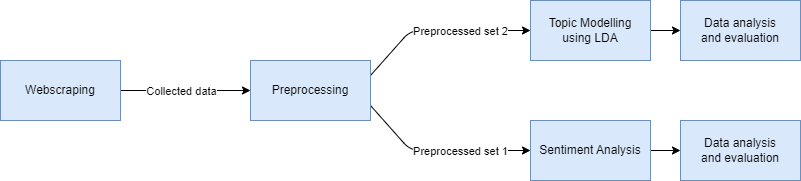
\includegraphics[width=0.8\textwidth]{resources/methodology.png}
    \caption{Summary of the methodology}
    \label{fig:methodology}
\end{figure}

The methodology can be divided into four steps: data collection via webscraping, the preprocessing of the collected data, the processing of the preprocessed data and the analysis along with the evaluation of the analysis. The processing step is further divided into two steps: topic modeling and sentiment analysis. The following sections will discuss each step in detail. 

%===========================================================
\subsection{Data Collection}

Data collection is a crucial step in any research. When conducting a text analysis, there is more often than not a need to collect data from the internet. The difficulty of this task can vary depending on the source of the data. For example, data from social media platforms or research portals is often easier to collect than data from websites. This is because these platforms often provide APIs that allow developers to collect data. On the other hand, other websites do not always provide APIs. In such cases, researchers may have to resort to webscraping. Webscraping is a method of automatically extracting, combining and saving data from websites. The paper uses webscraping to collect data from scamalert.sg.

\subsubsection{Scamalert}

Scamalert is a website run by the National Crime Prevention Council (NCPC), which is a non-profit organization that is committed promoting public awareness and concern about crime and to propagate the concept of self-help in crime prevention.~\citep{ncpc} Scamalert contains educational sources to help people protect themselves from scams as well as provide information about acting after falling victim to a scam.

Most relevant to this paper is the section "Scam Stories". Persons who experience a crime can share their stories on the website. The stories can be sent anonymously and are published on the website. The stories are well-formatted, all containing a title, date, category, and the story itself.

Scamalert does not provide an API to access the stories. Therefore, webscraping was used to collect the data. 

\subsubsection{Webscraping}

The webscraping process was done using four libraries in Julia. Julia is a contemporary programming language that is designed for high-performance computing which is favored among data scientists. % TODO: Add citation
The four libraries in use were:

\begin{itemize}
    \item HTTP.jl: A library for making HTTP requests and handling responses 
    \item Gumbo.jl: A library for parsing HTML documents
    \item Cascadia.jl: A library for querying HTML documents using CSS selectors
    \item JSON.jl: A library for parsing JSON documents
\end{itemize}

The first step of webscraping is figuring out the structure of the website to find an efficient way of scraping the data. Fortunately, the website was well-structured. The \texttt{/stories} directory contains all the pages with stories. The stories are paginated, with each page containing data about 6 stories. The pages contained a lot of meta data about the stories, but the most important were the following: title, date, category, URL and description of the story. The story itself is not included in the page. 

This meant that the webscraping needed to be done in two steps. The first step was to collect the meta data of the stories. This was done through POST requests using HTML.jl. The requests were then parsed into JSON documents using JSON.jl then saved locally on the computer. The second step was to collect the stories themselves. This was done by iterating through the JSON documents and collecting the URLs of the stories. The URLS were then used in GET requests to collect the HTML documents of the stories. The HTML documents were then parsed using Gumbo.jl. The stories were then extracted from the HTML documents using CSS selectors provided by Cascadia.jl. The stories were then saved locally on the computer.

The data was collected on the 10th of July 2023. On the first step, a total of 590 pages were scraped, containing a total of 3536 stories. It was observed later in the process that the requests did not contain the category of the scams. This was not remedied as the category was not considered for the analysis.

The second step retrieved 3495 stories, which is 41 stories less than expected. The process of scraping was logged. The logs have shown that there were 41 errors. The errors were not caused by connectivity issues, but rather by selector issues encountered by Cascadia.jl. Upon further investigation, it was found that the cause of the errors was the HTML documents themselves. The retrieved HTML documents contained an error that is likely caused by the website host deleting the story.

After the webscraping step, a decision was made to switch to Python as the choice for a programming language. While Julia does have many data analysis libraries, it was decided that Python's eco-system is more robust and enables more room for experimentation with the data. 

\subsubsection{Data Preprocessing}

Another important step of data analysis is the prepocessing of data. Data preprocessing can be defined as the cleaning of data and parsing it into a format that is suitable for further processing. An example of this is the removal of non-english stories, since the analysis aims to only consider stories written in english. There were a total of 5 non-english stories. The stories were removed from the dataset.

Since the aim is to do a text analysis, it is necessary to use natural language processing (NLP). NLP combines aritificial intelligence and linguistics to enable "understanding" of content. NLP is critical for topic models, as it is used to bring the text into a format that is suitable for topic modeling. Preprocessing also increases the accuracy of both topic models and sentiment analyses.~\cite{haddi2013role}\cite{chauhan2021topic}

The preprocessing was done using the Natural Language Toolkit (NLTK) library. Using NLTK, the text was tokenized, stripped off of punctuation, numbers, stopwords and emojis. Then the data was split into two sets: a set with lemmatizing and a set without lemmatizing. Lemmatizing is the process of reducing words to their root form. For instance, the word "writing" is reduced to "write". While lemmatization is a common preprocessing step, the decision to split the data was made on the basis of the claim that lemmatization correlates negatively with human interprability of topic models. An example of a sentence that is preprocessed is illustrated in the table below:


\begin{table}[h]
    \centering
    \begin{tabular}{cc}
        Original & Preprocessed \\ \hline
        I was scammed by a fake website. & scam fake website \\
        \\
        Original & Preprocessed (without lemmatization) \\ \hline
        I was scammed by a fake website. & scammed fake website \\
    \end{tabular}
    \caption{Example of a preprocessed sentence. The word "scammed" was not returned to its root form in the second table.}
    \label{tab:preprocessing}
\end{table}





%===========================================================
\subsection{Data Analysis}

%===========================================================
\subsection{Topic Modelling}
\subsubsection{Latent Dirichlet Allocation (LDA)}
\subsubsection{Parameter Tuning}
\subsubsection{Limitations}
%===========================================================
\subsection{Sentiment Analysis}
\subsubsection{Limitations}

%===========================================================
\section{Results}
\subsection{Topic Modeling}
\subsubsection{Evaluation}
\subsection{Sentiment Analysis}
\subsubsection{Evaluation}

%===========================================================

\section{Discussion}
\subsection{Summary}
\subsection{Interpretation}
\subsection{Limitations}
\subsection{Future Research}
\subsection{Conclusion}


%===========================================================
% References
%===========================================================
\pagebreak
\bibliographystyle{plain}
\bibliography{bibliography.bib}



%===========================================================
\pagebreak\noindent
\textbf{\LARGE Erkl\"arung}
\addcontentsline{toc}{section}{Declaration}

\bigskip\bigskip
\noindent 
I hereby confirm that I have independently written the 
bachelor's thesis and have not used any sources or aids 
other than those specified.
\bigskip
\noindent
% Date of Declaration

\bigskip\bigskip\bigskip
\noindent
% Automatic date
D\"usseldorf, \today \\
(Mundher Al-Ahmadi)

% bibliography
% \bibliographystyle{plain}



\end{document}